% Usefull codes

%\begin{figure}T_
%	\centering 
%	\includegraphics[width=0.5\columnwidth]{swallow.jpg}
%	\caption{Closed-Loop system with PID controller} 
%\label{fig:1} 
%\end{figure}
%
%\begin{enumerate}
%	\item Step input tracking
%	\item Changing reference tracking (Servo)
%	\item Disturbance rejection
%\end{enumerate}
%
%\begin{enumerate}[(\itshape a\normalfont)] % Sub-questions styled as italic letters
%	\item Suppose ``chuck" implies throwing.
%	\item Suppose ``chuck" implies vomiting.
%\end{enumerate}
%
%\begin{center}{\begin{minipage}{0.85\linewidth}
%\begin{lstlisting}[
%	caption={First-degree with time delay approximation},
%	captionpos=t,label={code:1}]
%system = tf(1,[1,9,23,15]);
%[y,t] = step(system);
%
%time_step = t(2)-t(1);
%u = ones(size(y));
%data = iddata(y,u,time_step);
%system_model = procest(data,'P1D');
%\end{lstlisting}
%\end{minipage}}\end{center}
%
%\begin{equation}
%	P(A|B) = \frac{P(B|A)P(A)}{P(B)}
%\label{eq:bayes}
%\end{equation}
%
%	\lstinputlisting[
%		caption=Luftballons Perl Script, % Caption above the listing
%		label=lst:luftballons, % Label for referencing this listing
%		language=Perl, % Use Perl functions/syntax highlighting
%		frame=single, % Frame around the code listing
%		showstringspaces=false, % Don't put marks in string spaces
%		numbers=left, % Line numbers on left
%		numberstyle=\tiny, % Line numbers styling
%	]{luftballons.pl}
%
%\begin{center}
%	\begin{tabular}{l l l}
%		\toprule
%		\textit{Per 50g} & Pork & Soy \\
%		\midrule
%		Energy & 760kJ & 538kJ\\
%		Protein & 7.0g & 9.3g\\
%		Carbohydrate & 0.0g & 4.9g\\
%		Fat & 16.8g & 9.1g\\
%		Sodium & 0.4g & 0.4g\\
%		Fibre & 0.0g & 1.4g\\
%		\bottomrule
%	\end{tabular}
%\end{center}
%
%\begin{table}[hbt]
%\caption{Genetic Algorithm Hyper-Parameters}
%\centering
%\begin{tabular}{l|c}
%\toprule
%Chromosome per generation & $100$ \\
%Encoding & Real \\
%Variables & $K_p,T_i,T_d$ \\
%Lower bounds & $[0, 0.001, 0]$ \\
%Upper bounds & $[200, 5, 0.8]$ \\
%Termination criteria & MaxGen=$300$ \\
%Selection technique & Stochastic uniform \\
%Crossover operation & Arithmatic \\
%Mutation probability & 0.01 \\
%\bottomrule
%\end{tabular}
%\label{tab:1}
%\end{table}
%
%\begin{figure}
%\centering
%\subfloat[Output y]{\includegraphics[width=0.75\columnwidth]{y3.eps}}\quad
%\subfloat[Control signal u]{\includegraphics[width=0.75\columnwidth]{u3.eps}}
%\caption[Simulation results of disturbance rejection]{Simulation results of disturbance rejection}
%\label{fig:1}
%\end{figure}

%----------------------------------------------------------------------------------------

\documentclass[
	12pt, % Default font size, values between 10pt-12pt are allowed
	%letterpaper, % Uncomment for US letter paper size
]{packages/fphw}

% packages

% template specific packages
\usepackage[utf8]{inputenc} % Required for inputting international characters
\usepackage[T1]{fontenc} % Output font encoding for international characters
%\usepackage{mathpazo} % Use the Palatino font

\usepackage{graphicx} % Required for including images

\usepackage{booktabs} % Required for better horizontal rules in tables

\usepackage{listings} % Required for insertion of code

\usepackage{enumerate} % To modify the enumerate environment


% my packages

\setlength\parindent{0pt}

%\usepackage[framed,numbered,autolinebreaks,useliterate]{packages/mcode}

\graphicspath{{Figures/}}

\usepackage{subfig} % Required for creating figures with multiple parts (subfigures)
\usepackage[table,xcdraw]{xcolor}
\usepackage{hyperref} % More descriptive referencing
\usepackage{xcolor}
\hypersetup{
    colorlinks,
    linkcolor={blue!50!black},
    citecolor={blue!50!black},
    urlcolor={blue!80!black}
}
\AtBeginDocument{\renewcommand{\ref}[1]{\autoref{#1}}}

\usepackage{float}

\usepackage{amsmath}

\definecolor{codegreen}{rgb}{0.25,0.5,0.5}
\definecolor{codegray}{rgb}{0.4,0.4,0.4}
\definecolor{codepurple}{rgb}{0.729,0.129,0.129}
\definecolor{backcolour}{rgb}{0.968,0.968,0.968}
\definecolor{rcolour}{rgb}{0.81,0.81,0.81}
\definecolor{impcolour}{rgb}{0,0.5,0}

\lstdefinestyle{mystyle}{
	language=Python,
	frame=single,
	framerule=1.5pt,
	rulecolor=\color{rcolour},
    backgroundcolor=\color{backcolour},   
    commentstyle=\color{codegreen},
    keywordstyle=\color{impcolour},
    numberstyle=\tiny\color{codegray},
    stringstyle=\color{codepurple},
    basicstyle=\ttfamily\footnotesize,
    breakatwhitespace=false,         
    breaklines=true,                 
    captionpos=t,                    
    keepspaces=true,                 
    numbers=left,                    
    numbersep=10pt,                  
    showspaces=false,                
    showstringspaces=false,
    showtabs=false,                  
    tabsize=4,
}

\lstset{style=mystyle}
\renewcommand{\lstlistingname}{In}

%----------------------------------------------------------------------------------------
%	ASSIGNMENT INFORMATION
%----------------------------------------------------------------------------------------

\title{Final Project Report} % Assignment title

\author{Armin Ghanbarzadeh, Yasamin Borhani, Mohammad Hoseinzadeh} % Student name

\date{23 Jan, 2022} % Due date

\institute{K. N. Toosi University of Technology\\ Faculty of Mechanical Engineering - Mechatronics Group } % Institute or school name

\class{IoT} % Course or class name

\instructor{Dr. Najafi} % Professor or teacher in charge of the assignment

%----------------------------------------------------------------------------------------

\begin{document}

\maketitle 
The code can be found at \url{https://github.com/ghanbarzadeh/Course_MachineVision_2021/blob/master/CHW4.ipynb}.
%----------------------------------------------------------------------------------------
\section*{Preprocessing Camera Images}

\subsection*{Loading and Comparing Left \& Right Images}

\begin{center}{\begin{minipage}{0.9\linewidth}
\begin{lstlisting}[language=Python, basicstyle=\fontsize{8}{10}\selectfont\ttfamily]
import numpy as np
import cv2 as cv
import matplotlib.pyplot as plt

# Read both images and convert to grayscale
img1 = cv.imread('left_img.png', cv.IMREAD_GRAYSCALE)
img2 = cv.imread('right_img.png', cv.IMREAD_GRAYSCALE)

# ------------------------------------------------------------
# PREPROCESSING

# Compare unprocessed images
fig, axes = plt.subplots(1, 2, figsize=(15, 10))
axes[0].imshow(img1, cmap="gray")
axes[1].imshow(img2, cmap="gray")
axes[0].axhline(250)
axes[1].axhline(250)
axes[0].axhline(450)
axes[1].axhline(450)
plt.suptitle("Original images")
plt.show()
\end{lstlisting}
\end{minipage}}\end{center}

Running this shows us the left and right images with the lines $y=250$ and $y=450$.

\begin{figure}[H]
\centering
\subfloat{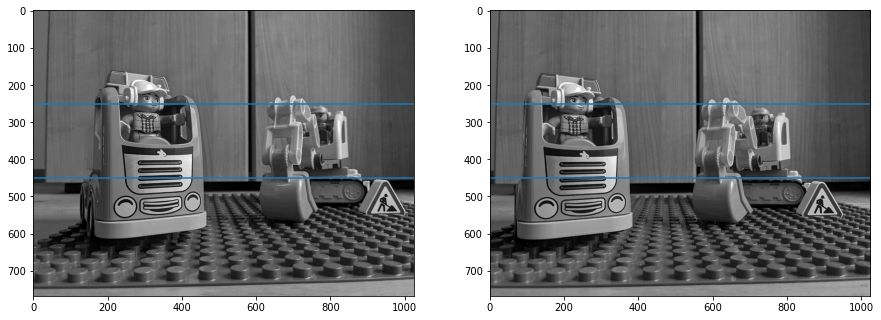
\includegraphics[width=0.98\columnwidth]{1}}
\caption{Comparing Left \& Right Images}
\end{figure}

\subsection*{Wrapping Images for Stereo Rectification}

We must first detect suitable keypoints. 

\begin{center}{\begin{minipage}{0.9\linewidth}
\begin{lstlisting}[language=Python, basicstyle=\fontsize{8}{10}\selectfont\ttfamily]
# Initiate SIFT detector
sift = cv.SIFT_create()
# find the keypoints and descriptors with SIFT
kp1, des1 = sift.detectAndCompute(img1, None)
kp2, des2 = sift.detectAndCompute(img2, None)

# Visualize keypoints
imgSift = cv.drawKeypoints(
    img1, kp1, None, flags=cv.DRAW_MATCHES_FLAGS_DRAW_RICH_KEYPOINTS)
cv2_imshow(imgSift)
\end{lstlisting}
\end{minipage}}\end{center}

\begin{figure}[H]
\centering
\subfloat{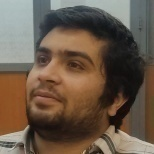
\includegraphics[width=0.78\columnwidth]{2}}
\caption{Found Keypoint using SIFT}
\end{figure}

We can now match keypoints to use for stereo rectification. 

\begin{center}{\begin{minipage}{0.9\linewidth}
\begin{lstlisting}[language=Python, basicstyle=\fontsize{8}{10}\selectfont\ttfamily]
# Match keypoints in both images
FLANN_INDEX_KDTREE = 1
index_params = dict(algorithm=FLANN_INDEX_KDTREE, trees=5)
search_params = dict(checks=50)   # or pass empty dictionary
flann = cv.FlannBasedMatcher(index_params, search_params)
matches = flann.knnMatch(des1, des2, k=2)

# Keep good matches: calculate distinctive image features
matchesMask = [[0, 0] for i in range(len(matches))]
good = []
pts1 = []
pts2 = []

for i, (m, n) in enumerate(matches):
    if m.distance < 0.7*n.distance:
        # Keep this keypoint pair
        matchesMask[i] = [1, 0]
        good.append(m)
        pts2.append(kp2[m.trainIdx].pt)
        pts1.append(kp1[m.queryIdx].pt)
        
# Visualizing keypoints between two images
draw_params = dict(matchColor=(0, 255, 0),
                   singlePointColor=(255, 0, 0),
                   matchesMask=matchesMask[300:500],
                   flags=cv.DrawMatchesFlags_DEFAULT)

keypoint_matches = cv.drawMatchesKnn(
    img1, kp1, img2, kp2, matches[300:500], None, **draw_params)
cv2_imshow(keypoint_matches)
\end{lstlisting}
\end{minipage}}\end{center}

\begin{figure}[H]
\centering
\subfloat{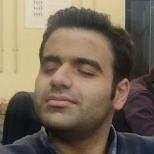
\includegraphics[width=0.98\columnwidth]{3}}
\caption{Best matched keypoints}
\end{figure}

Fundamental Matrix calculation code

\begin{center}{\begin{minipage}{0.9\linewidth}
\begin{lstlisting}[language=Python, basicstyle=\fontsize{8}{10}\selectfont\ttfamily]
pts1 = np.int32(pts1)
pts2 = np.int32(pts2)
fundamental_matrix, inliers = cv.findFundamentalMat(pts1, pts2, cv.FM_RANSAC)

# We select only inlier points
pts1 = pts1[inliers.ravel() == 1]
pts2 = pts2[inliers.ravel() == 1]
\end{lstlisting}
\end{minipage}}\end{center}

Visualizing Epilines:

\begin{center}{\begin{minipage}{0.9\linewidth}
\begin{lstlisting}[language=Python, basicstyle=\fontsize{8}{10}\selectfont\ttfamily]
# Visualize epilines
# Adapted from: https://docs.opencv.org/master/da/de9/tutorial_py_epipolar_geometry.html
def drawlines(img1src, img2src, lines, pts1src, pts2src):
    ''' img1 - image on which we draw the epilines for the points in img2
        lines - corresponding epilines '''
    r, c = img1src.shape
    img1color = cv.cvtColor(img1src, cv.COLOR_GRAY2BGR)
    img2color = cv.cvtColor(img2src, cv.COLOR_GRAY2BGR)
    # Edit: use the same random seed so that two images are comparable!
    np.random.seed(0)
    for r, pt1, pt2 in zip(lines, pts1src, pts2src):
        color = tuple(np.random.randint(0, 255, 3).tolist())
        x0, y0 = map(int, [0, -r[2]/r[1]])
        x1, y1 = map(int, [c, -(r[2]+r[0]*c)/r[1]])
        img1color = cv.line(img1color, (x0, y0), (x1, y1), color, 1)
        img1color = cv.circle(img1color, tuple(pt1), 5, color, -1)
        img2color = cv.circle(img2color, tuple(pt2), 5, color, -1)
    return img1color, img2color


# Find epilines corresponding to points in right image (second image) and
# drawing its lines on left image
lines1 = cv.computeCorrespondEpilines(
    pts2.reshape(-1, 1, 2), 2, fundamental_matrix)
lines1 = lines1.reshape(-1, 3)
img5, img6 = drawlines(img1, img2, lines1, pts1, pts2)

# Find epilines corresponding to points in left image (first image) and
# drawing its lines on right image
lines2 = cv.computeCorrespondEpilines(
    pts1.reshape(-1, 1, 2), 1, fundamental_matrix)
lines2 = lines2.reshape(-1, 3)
img3, img4 = drawlines(img2, img1, lines2, pts2, pts1)

plt.subplot(121), plt.imshow(img5)
plt.subplot(122), plt.imshow(img3)
plt.show()
\end{lstlisting}
\end{minipage}}\end{center}

\begin{figure}[H]
\centering
\subfloat{
\includegraphics[width=0.98\columnwidth]{4}}
\caption{Epilines}
\end{figure}

\section*{Stereo Rectification}

\begin{center}{\begin{minipage}{0.9\linewidth}
\begin{lstlisting}[language=Python, basicstyle=\fontsize{8}{10}\selectfont\ttfamily]
# Stereo rectification (uncalibrated variant)
h1, w1 = img1.shape
h2, w2 = img2.shape
_, H1, H2 = cv.stereoRectifyUncalibrated(
    np.float32(pts1), np.float32(pts2), fundamental_matrix, imgSize=(w1, h1)
)
\end{lstlisting}
\end{minipage}}\end{center}

Visualizing the images after rectification

\begin{center}{\begin{minipage}{0.9\linewidth}
\begin{lstlisting}[language=Python, basicstyle=\fontsize{8}{10}\selectfont\ttfamily]
img1_rectified = cv.warpPerspective(img1, H1, (w1, h1))
img2_rectified = cv.warpPerspective(img2, H2, (w2, h2))
cv.imwrite("rectified_1.png", img1_rectified)
cv.imwrite("rectified_2.png", img2_rectified)
fig, axes = plt.subplots(1, 2, figsize=(15, 10))
axes[0].imshow(img1_rectified, cmap="gray")
axes[1].imshow(img2_rectified, cmap="gray")
axes[0].axhline(250)
axes[1].axhline(250)
axes[0].axhline(450)
axes[1].axhline(450)
# plt.suptitle("Rectified images")
plt.savefig("rectified_images.png")
plt.show()
\end{lstlisting}
\end{minipage}}\end{center}

\begin{figure}[H]
\centering
\subfloat{\includegraphics[width=0.98\columnwidth]{5}}
\caption{Rectified Images}
\end{figure}
%----------------------------------------------------------------------------------------
%------------------------------------------------

\end{document}
